\documentclass[openany]{book}
\usepackage[utf8]{inputenc}
\usepackage{graphicx}
\usepackage{amsmath}
\usepackage[a4paper, total={6in, 8in}]{geometry}

\renewcommand{\baselinestretch}{1.3}

\title{Learning Depth and Visual Odometry From Light Fields \\
\large AMME4111 Thesis A Progress Report}

\author{Joseph Daniel}
\date{November 2019}

\begin{document}

\maketitle

\tableofcontents

\chapter{Introduction}
Humans have a remarkable ability to perceive visual stimuli emanating from the world around them. Not only do we identify different objects, scene depth, movement, and colour with ease, but we often draw meaning and even enjoyment from the combination of light rays bouncing around space and arriving at our eyes. We are able to automatically compensate for differences in lighting and viewing angle, and we can extract complex information such as emotion from what we process visually. To word it concisely, the human visual perception system is one of the most versatile and robust image processing machines that we know of. Most man-made machines on the other hand are much more easily decomposed into a set of deterministic modules that require explicit, well defined instruction sets. Often, when given an image, there is no straightforward function that directly maps from pixel intensities to the semantic meaning of that image. As researchers tackling problems in computer vision, we are usually interested in developing the algorithms that can help machines not only sense the world, but perceive it in a way that is useful. The objective of this thesis project is to develop a pipeline that simultaneously learns to perform two tasks. The first is visual odometry - the act of estimating camera motion from a sequence of images. The growth of autonomous robotics has meant that there is an ever-growing need for accurate navigation and localisation when satellite positioning is unavailable or wheel encoder odometry is unreliable. An autonomous unmanned aerial vehicle (UAV) navigating an unknown indoor environment is one example where visual odometry is a valuable feedback signal that can be used to precisely control its position. The second is depth estimation, that is, discerning the distance of objects in a scene from the imaging device. The ability to perform depth estimation from visual cues is desirable in applications such as autonomous vehicles where navigating new environments whilst avoiding collisions is a basic requirement. Being able to draw depth information from a camera sensor will help to enable these capabilities, especially in applications where methods such as Lidar or RGBD sensors are prohibitive - small quad-copters and internal medical imaging devices are examples where this might be the case.


Humans are exceptionally well adapted to these tasks - our two eyes allow us to process the 3D geometry of the scene, while our learned experiences are often able to fill in the gaps where geometric information is insufficient or unavailable. Unfortunately, image processing algorithms are not equipped with this same kind of human intuition, and so the deceptively complex task of estimating the 3D structure of a scene from a sequence of images continues to attract attention from the computer vision community. 


The price of camera components is decreasing while image quality continues to improve, not only making cameras an attractive perception module for autonomous robotics, but also spurring the popularity of multiple-view imaging. Embracing this idea, this thesis project seeks to develop a pipeline that performs these tasks by taking advantage of the rich geometric information exposed when using multiple views. Thus, this thesis project adopts the vocabulary and the concepts from the area of light field imaging. More broadly however, the principle underpinning much of this thesis is that novel imaging devices that break away from the traditional pinhole model of the camera have vast implications in the field of machine vision. We can draw inspiration from the animal kingdom, where the biological eye, having evolved independently no fewer than 50 times has been found in a huge variety of configurations, adapted to their particular set of challenges and environments. Most cameras are modeled after one particular variation - the human eye. When we take a photograph, we like to be reminded of what was visible to us, and so cameras are built to capture a rich, but realistic view of the world. An important question in computer vision is then, what is the best kind of camera to choose given a particular set of tasks and challenges in robotics? In this thesis project a camera array, a simple yet versatile extension of the stereo camera will be investigated as one such choice.


Another core objective of this thesis is to develop a pipeline that relies principally on unsupervised machine learning models to perform the two tasks side-by-side. This approach is chosen with the intention that a data-driven model can build a robustness to scenarios that are difficult to design for using hand crafted solutions.  Furthermore, this pipeline will benefit from being self-supervised - unlike data-driven models that require direct supervision from labelled data to improve their performance, this pipeline has no intermediary requirements between the data collection and training routines. Not only does this mean that the expensive process of hand-labelling data is unnecessary for this pipeline to function, but the model will be able to continue learning, benefiting from new data collected in situ. An adaptive perception module that learns to operate effectively in new environments is a desirable capability in robotics, especially when considering that effects such as thermal expansion, vibration and shocks can frequently render our equipment calibrations meaningless in the field. 

In this progress report we will first establish the conceptual groundwork that this thesis builds upon with a discussion surrounding the seminal texts that have shaped the state-of-the-art literature in visual odometry and depth estimation. In understanding those texts, we demonstrate that existing methods have yielded excellent results, whilst identifying that there is a substantial potential for improvement on state-of-the-art results using multi-view imaging devices. 



\chapter{Background}

\section{Geometry in Computer Vision}

The pixel is the building block of digital imagery. Thanks to our ability to fabricate advanced circuits on the scale of nanometers, digital camera sensors have become ubiquitous - making their way into all manner of consumer devices. Because the photodiodes in camera sensors are typically arranged on a 2D plane, most of our operations on digital images manipulate the 2D structures present in that pixel data. However, it is important to remember that the 2D shapes and structures that appear on the sensor plane are projected versions of a 3D world. 

\subsection{The Pinhole Camera}

The most basic kind of camera, the pinhole camera projects a 3D world point $(X, Y, Z)$ to a homogenous coordinate on a 2D plane $(u, v, w)$. This relationship is captured in the $3 \times 3$ camera intrinsics matrix, and is typically written as 

\begin{equation}
\begin{bmatrix}
    u\\
    v\\
    w
\end{bmatrix} = 
\begin{bmatrix}
    f_x & s & u_0 \\ 
    0 & f_y  & v_0 \\ 
    0 & 0 & 1 
\end{bmatrix}
\begin{bmatrix}
    X \\
    Y \\
    Z
\end{bmatrix}
\end{equation}


\begin{figure}[htbp]
    \centering 
    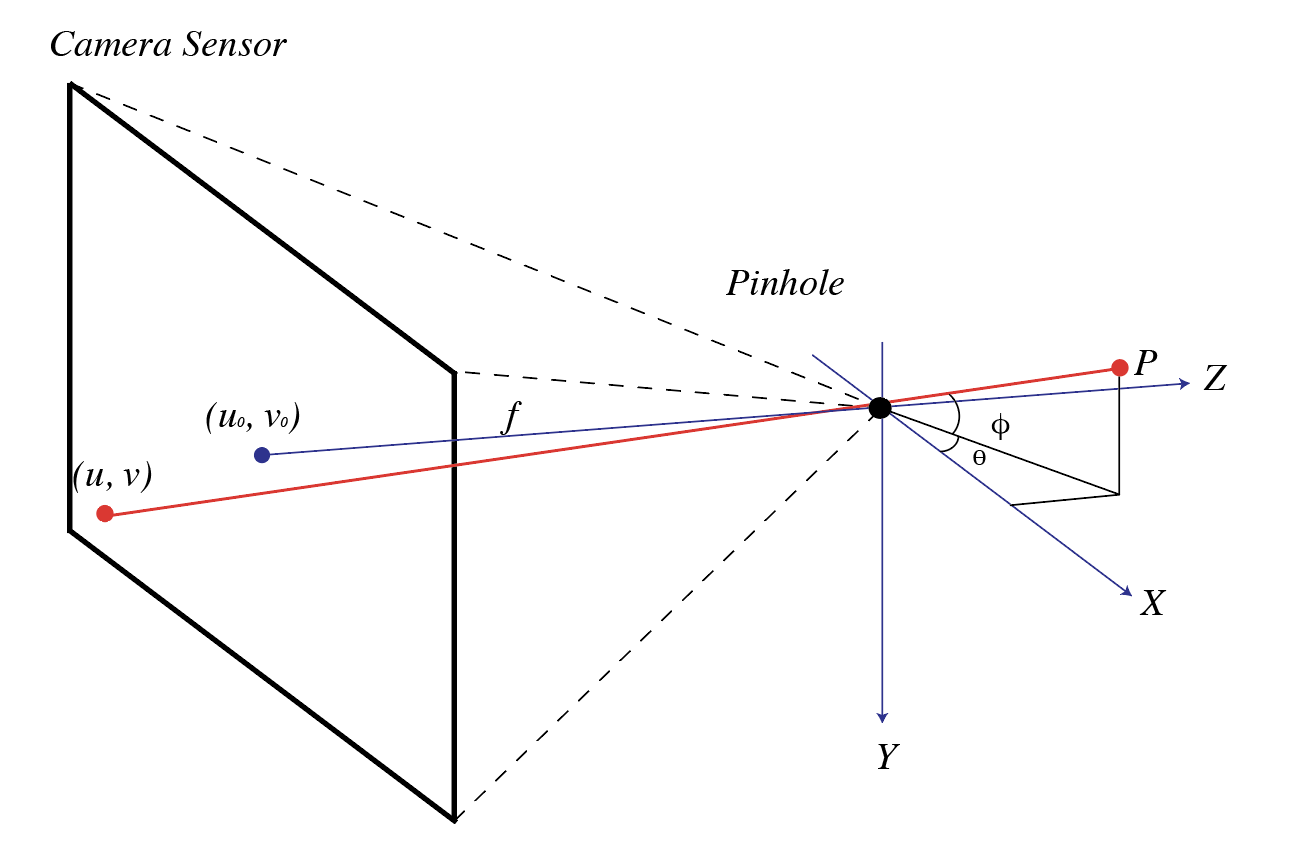
\includegraphics[width=4in]{images/pinhole.png}
    \caption{The pinhole model describes how a light ray originating from world coordinate $P$ is received at pixel coordinate $(u, v)$. Equivalently, the pinhole model can be thought of as associating the light ray of elevation $\phi$ and azimuth $\theta$ with the specific pixel coordinate $(u, v)$. Since the relationship is a one-to-one mapping between ray directions and pixel coordinates, the inverse of the intrinsics matrix $K^{-1}$ associates each pixel with a corresponding ray direction.}
\end{figure}

The intrinsics matrix can alternatively be thought of as mapping ray directions to pixel coordinates:

\begin{equation}
    \begin{bmatrix}
        u\\
        v\\
        1
    \end{bmatrix} = 
    \begin{bmatrix}
        f_x & s & u_0 \\ 
        0 & f_y  & v_0 \\ 
        0 & 0 & 1 
    \end{bmatrix}
    \begin{bmatrix}
        tan(\theta) \\
        tan(\phi) \\
        1
    \end{bmatrix}
    \end{equation}


\subsection{Epipolar Geometry and the Fundamental Matrix}

Epipolar geometry describes the relationship between two cameras, and imposes a set of constraints which makes it possible for us to draw meaningful geometric information when we have two views of the same scene. This relationship is encapsulated in a $3 \times 3$ matrix called the Fundamental matrix $F$. The culmination of the epipolar constraint is that any point in 3 dimensional space that appears at pixel $(u_1, v_1, 1)$ in one view and $(u_2, v_2, 1)$ in the second view must satisfy the relationship:

\begin{equation}
    \begin{bmatrix}
        u_1, v_1, 1
    \end{bmatrix}^T
    F
    \begin{bmatrix}
        u_2, v_2, 1
    \end{bmatrix}
    = 0
\end{equation}

\begin{figure}
    \centering
    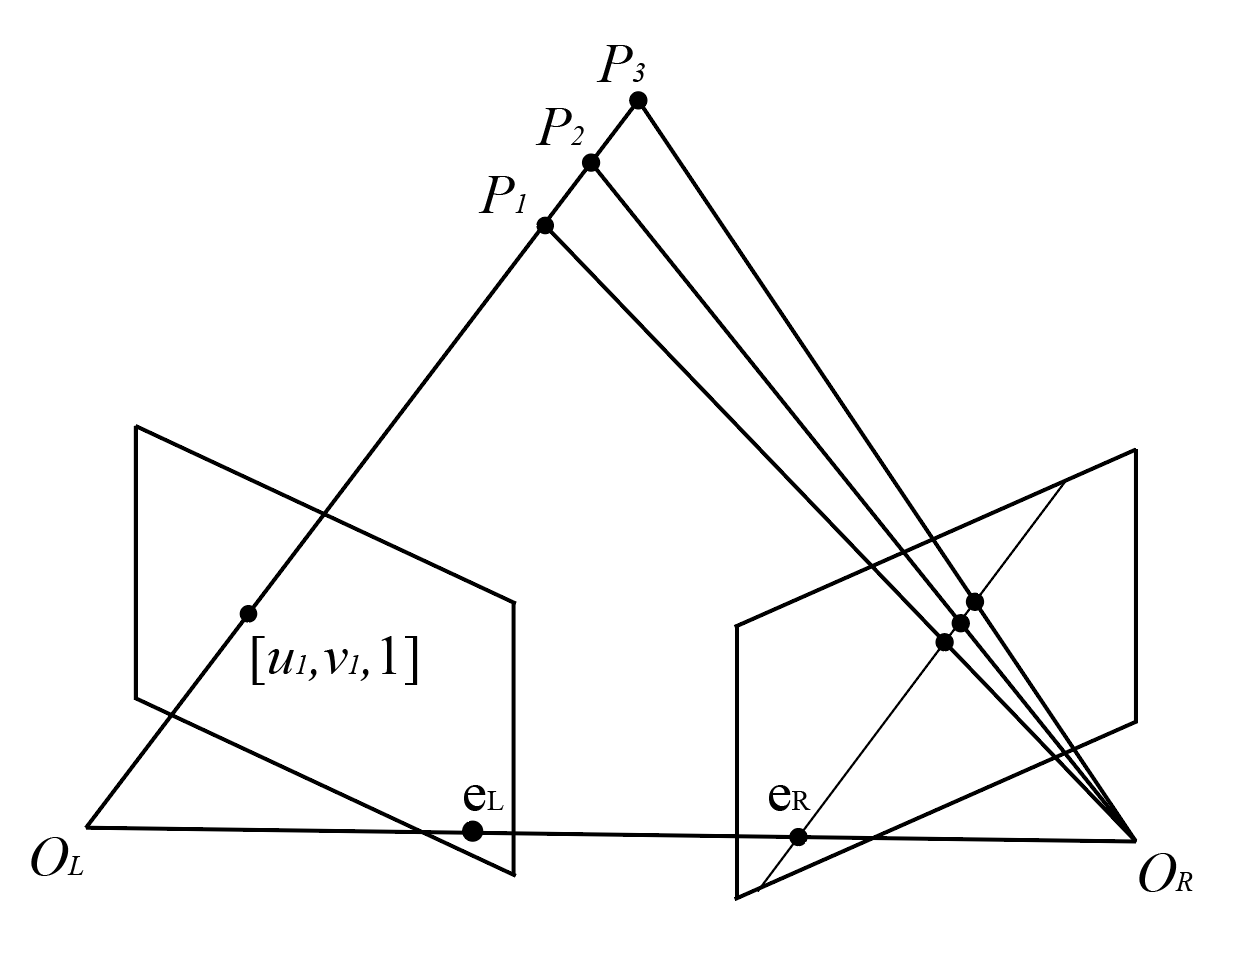
\includegraphics[width=3in]{images/epipolarplane.png}
    \caption{Epipolar geometry is the geometry of stereo camera pairs. The point $[u,v,1]$ can be projected to any number of points $P1, P2, P3, ... $, however any one of these points will be seen by camera 2 along the epipolar line. Practically, this simplifies a search for image-to-image correspondences to a 1D search.}
    \label{epipolarplane}
\end{figure}

The Fundamental matrix thus describes the rotation and translation between two cameras up to scale. Any point projected from pixel coordinate $(u_1, v_1, 1)$ must lie on the epipolar line in the second image, which is formed by the intersection of the epipolar plane and the imaging plane. 




\section{The 4D Light Field}
Light field imaging has emerged as a powerful tool in computer vision for robotics, offering a rich higher-dimensional representation than what can be captured by conventional optics. The underlying principle used to describe the light field is the plenoptic function, a 7-dimensional mapping that assigns radiance values to the light rays at every position in space, in every orientation, at all wavelengths, throughout all of time \cite{ihrke2016lfprinciples}. \cite{adelson1991plenoptic} shows that this can be formally expressed as $L(x,y,z,\theta, \phi, \lambda, t)$, and measured in $W/m^2/sr/nm/s$. 
With the addition of practical constraints however, the plenoptic function can be expressed more concisely as a parameterisation of 4 variables. 

Pixels on camera sensors integrate the number of photons arriving at them over a finite period of time removing the temporal dimension, and each colour channel can be thought of as a monochromatic sampling of the light field, removing the spectral dimension. Additionally, and importantly, is the constraint that the radiance of light rays propagating through a vacuum do not change if samples are restricted to the convex hull of the scene, thus reducing the overall dimensionality of the plenoptic function by one parameter \cite{levoy1996lfrendering}. To illustrate this, one could think of the light rays leaving the inside of a bowl sat upright on a table. Many of those rays may only travel a small distance before being blocked by the inside of the bowl itself, meaning those rays will never be registered by any practical measurement device. As shown in figure \ref{convexhull} if we consider only the convex hull of the bowl however, we are required only to represent the value of the plenoptic function on the encapsulating surface of the object \cite{gortler1996lumigraph}.

\begin{figure}[htbp]
    \centering
    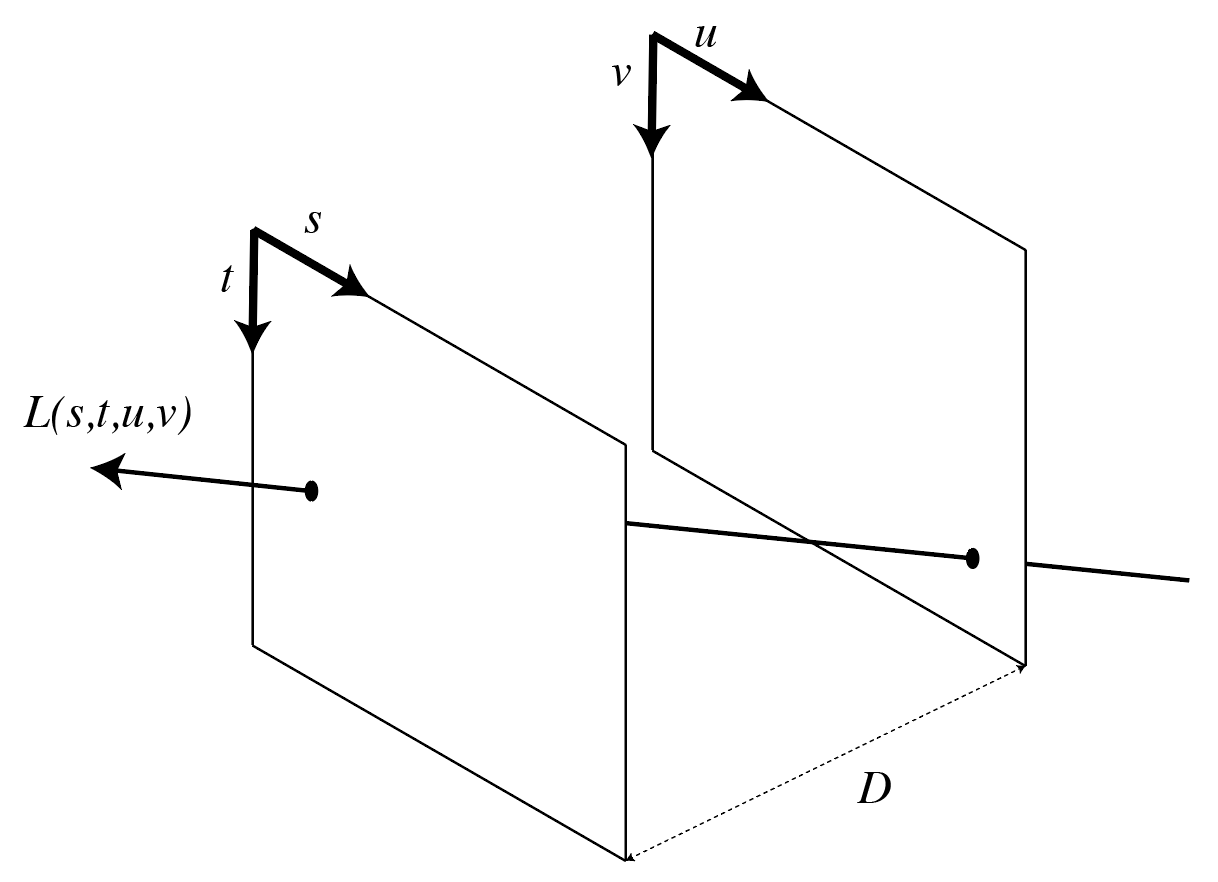
\includegraphics[width=2.5in]{images/2pp.png}
    
\includegraphics[width=0.3in]{images/blank.png}
    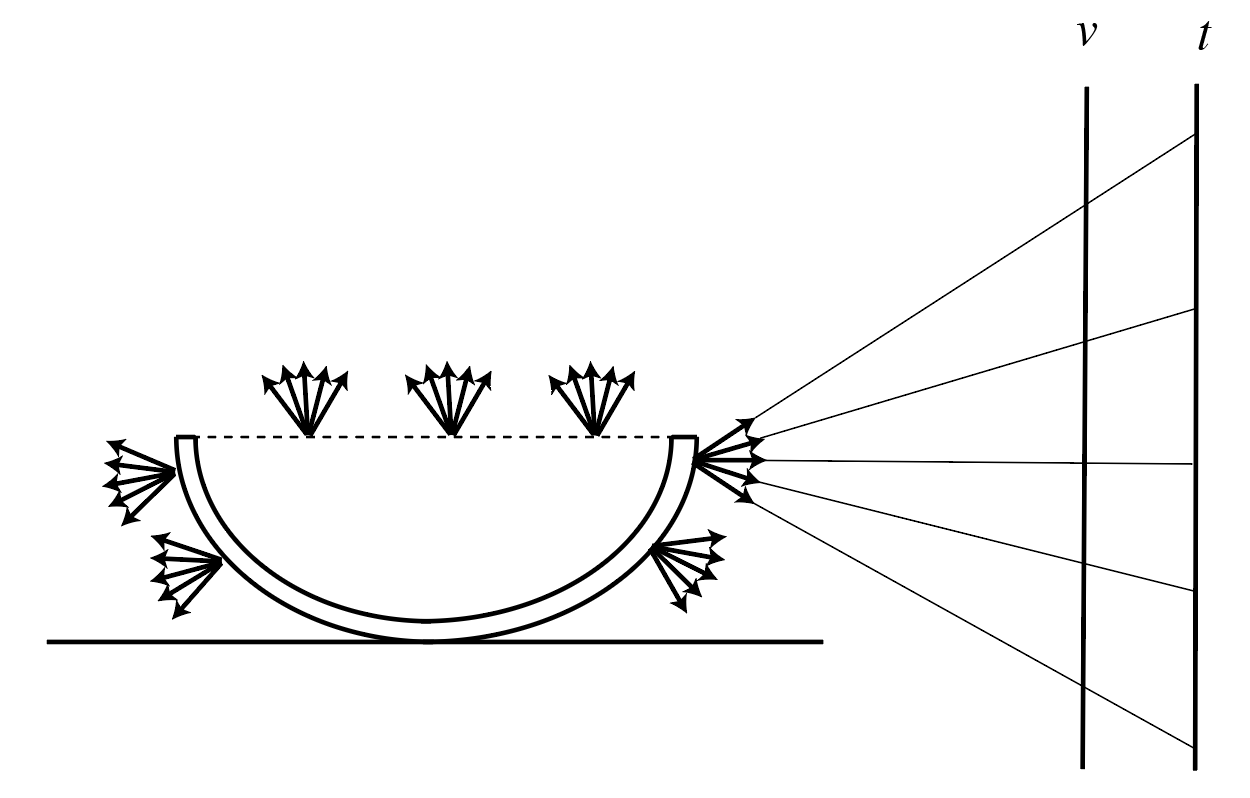
\includegraphics[width=2.5in]{images/convexhull.png}
    
    \caption{Two plane parameterisation (left): the plenoptic function can be described by the radiance along a ray passing through two parallel planes. The free space assumption (right): if we consider only the bundle of rays leaving from the convex hull of the object at a particular instance in time, in a single colour channel, we can parameterise the light rays as a function of 4 variables rather than 7.}
    
    \label{convexhull}
\end{figure}

Also illustrated is a common convention for describing light rays in this 4 dimensional space called the two plane parameterisation. In this parameterisation, two parallel planes are used to fix both the position and orientation of each ray by fixing their points of intersection with two parallel planes. By convention, the plane closest to the scene is termed \textit{u, v} and the plane closest to the camera sensor is the \textit{s, t} plane.

This 4D realisation of the light field originated as a model of rendering 3D computer graphics, one which shifted emphasis from notions of texture and geometric primitives to modeling the behaviour of light rays permeating space. Since then however, the conceptual framework of the light field has drawn a following of researchers at an intersecting region of signal processing, computer vision and robotics \cite{dansereau2014phd}. This notion of light field imaging finds a foothold in this thesis project through the utilisation of camera arrays, which are devices that sample multiple views of the same scene. Using a camera array is a simple method for acquiring a sparse sample of the light field, where the position of the camera determines \textit{(s,t)} while the location of the pixel determines \textit{(u, v)} \cite{yao2016camarray}. The images captured from a camera array are mapped easily to the 4D light field, and identifying corresponding pixels across images exposes a rich tapestry of geometric information about the scene. 


\begin{figure}[tbp]
    \centering
    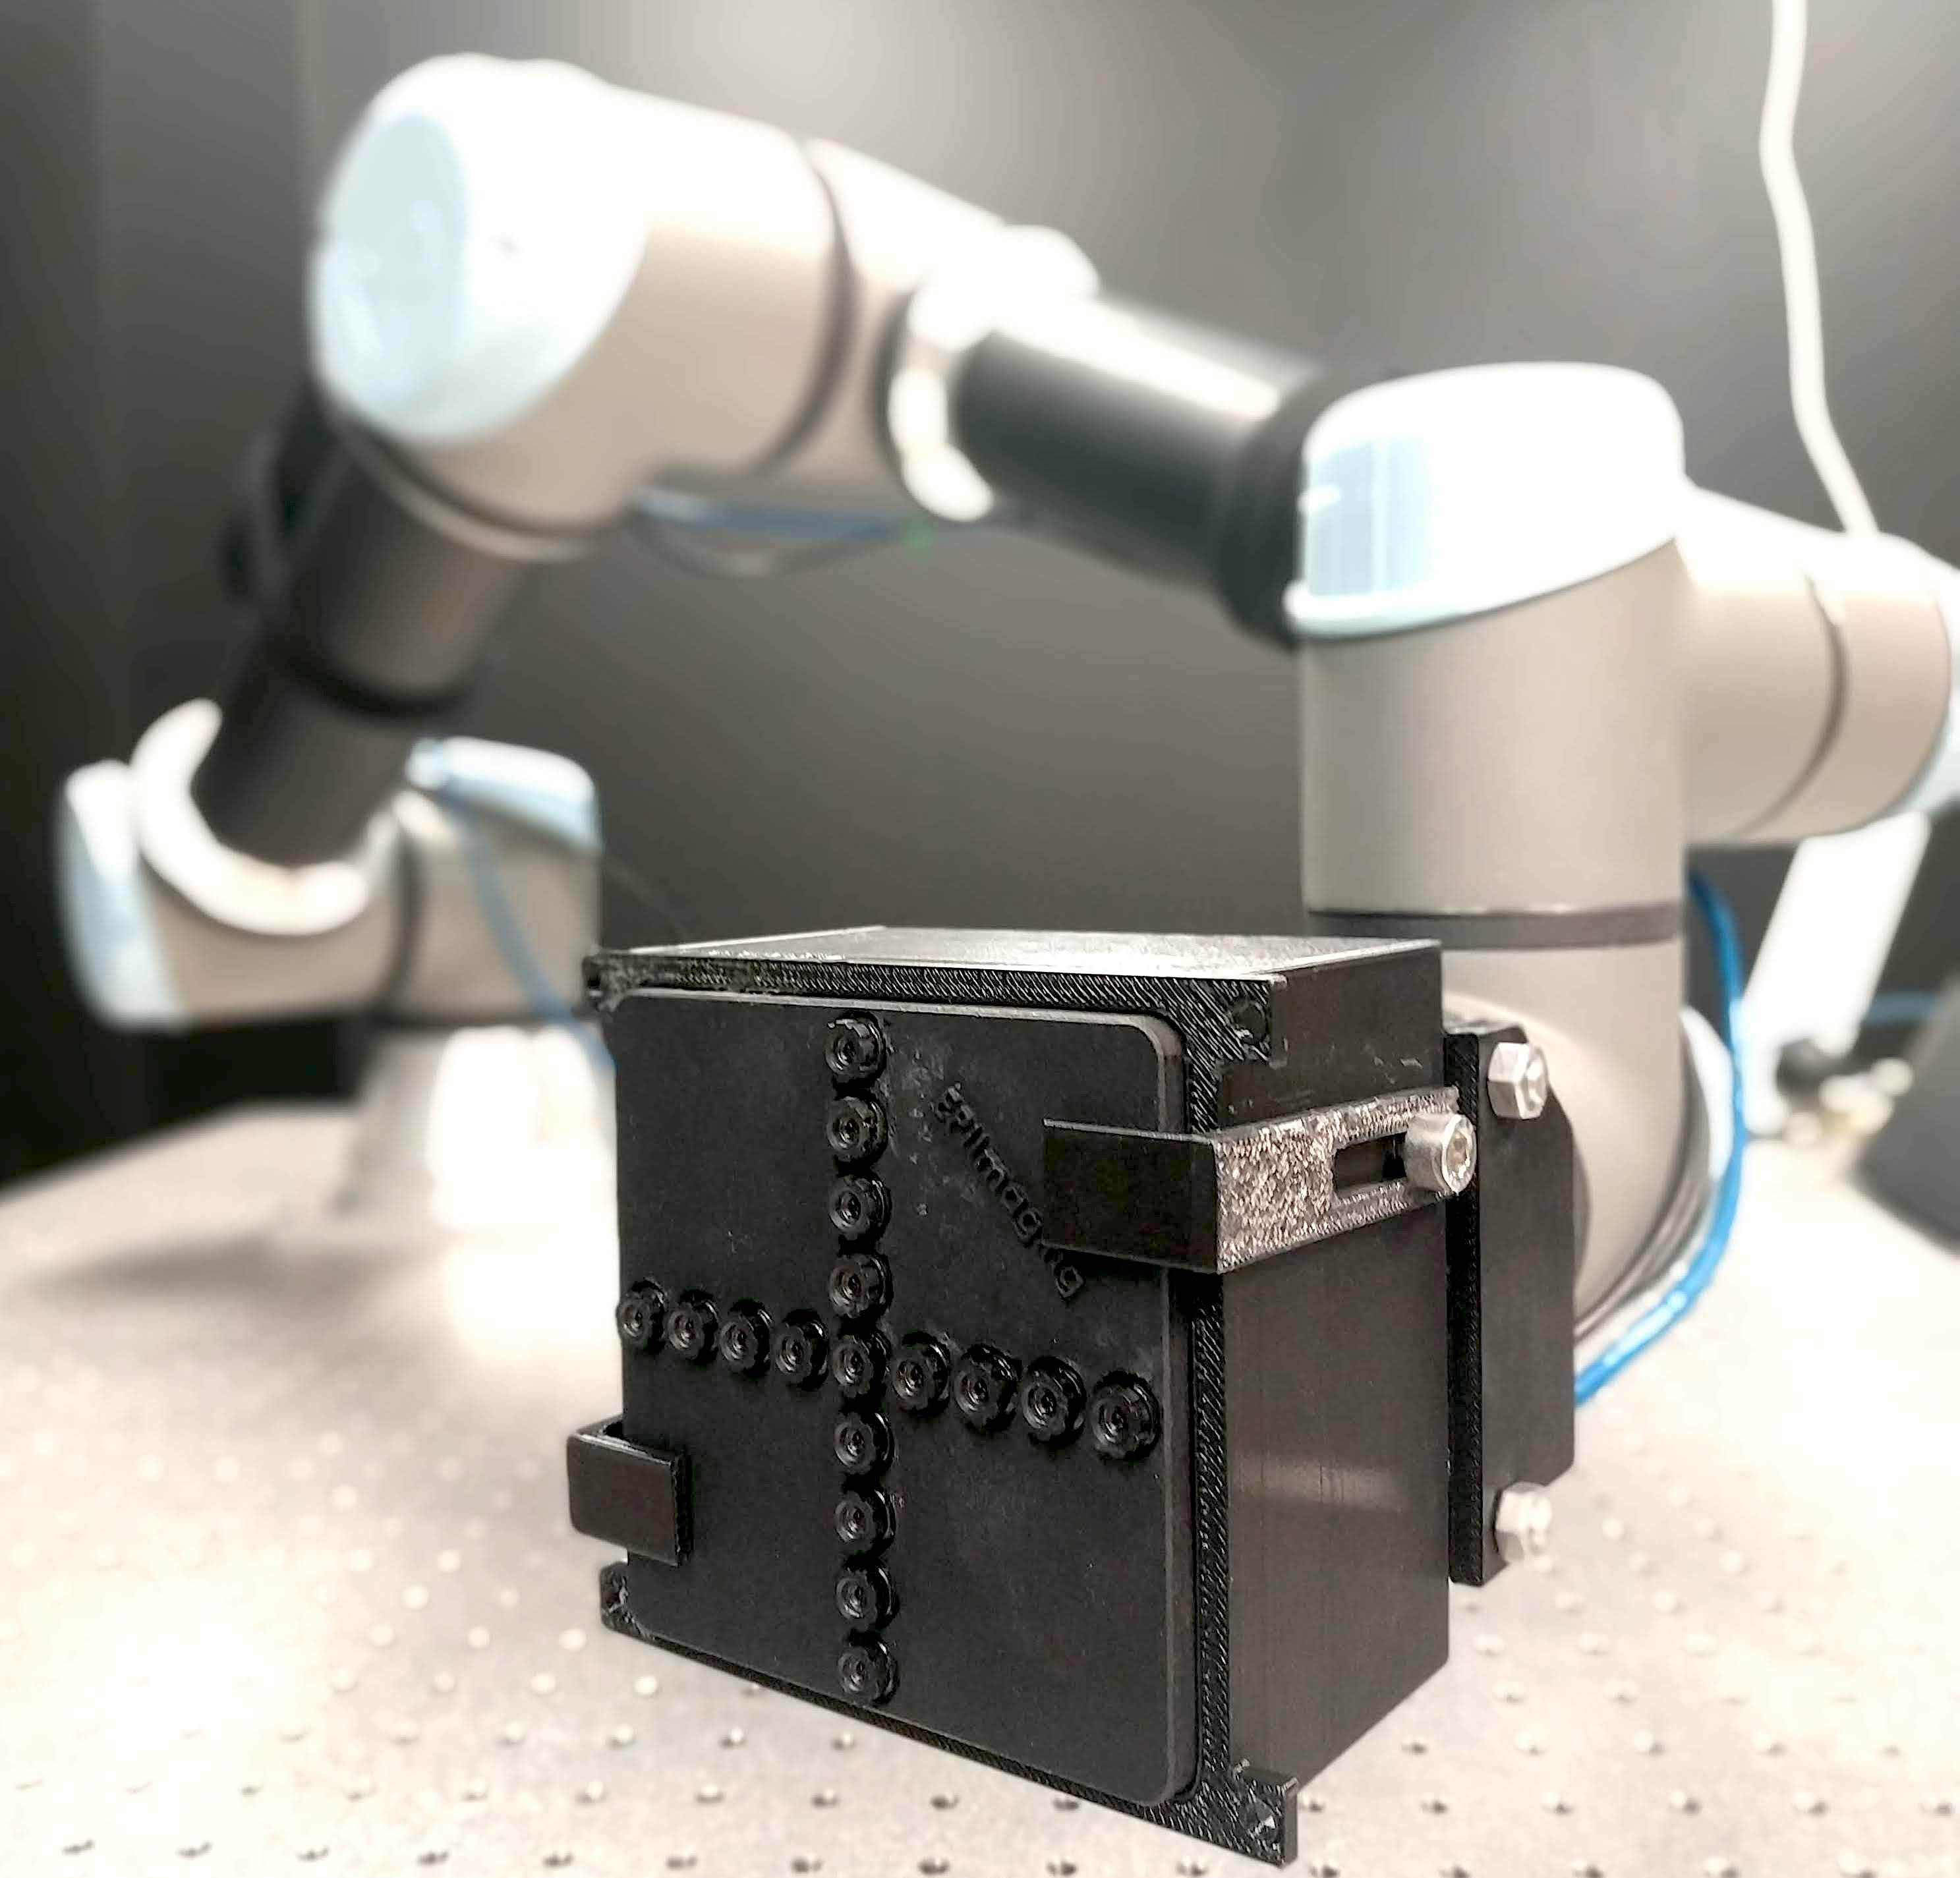
\includegraphics[width=4.5in]{images/robotcamera.jpg}
    \caption{An example of a camera array mounted on a robotic arm. This camera array is configured as 17 sub-apertures arranged on a single plane in a cross-hair formation. Camera arrays sample several views of the same scene and are thus capable of acquiring a sparse sample of the light field. This is the camera that will be used throughout this thesis project.}
    \label{cameraarray}
    \vspace{1cm}
    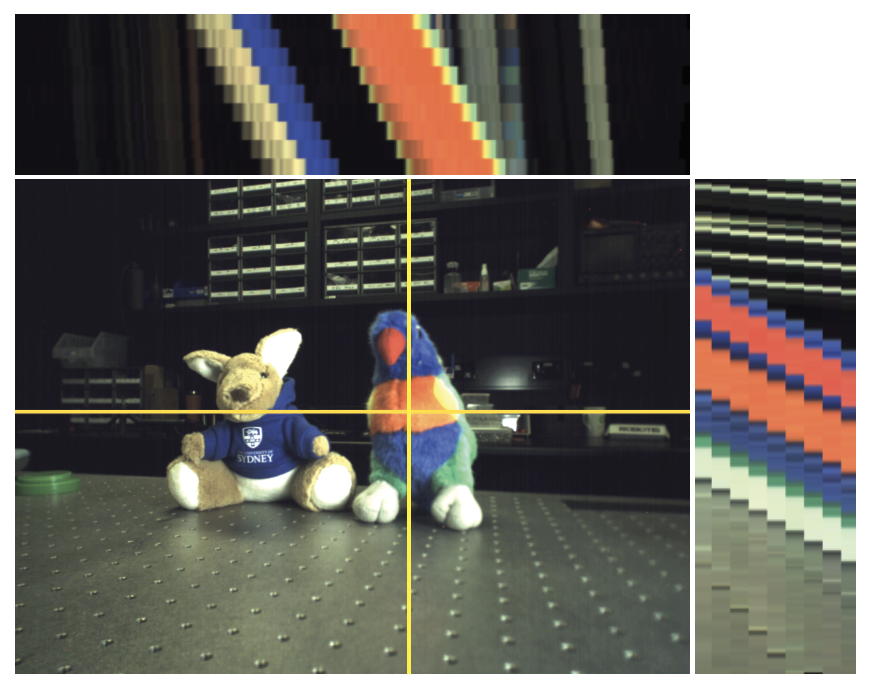
\includegraphics[width=1.6in]{images/epipolarimage.png}
    
\includegraphics[width=0.4in]{images/blank.png}
    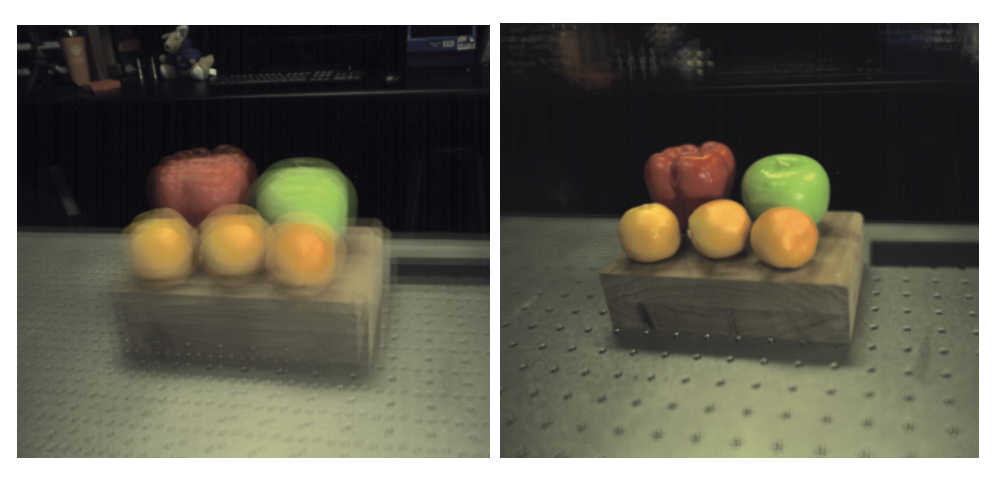
\includegraphics[width=3.5in]{images/fruitfocus.png}
    \caption{Epipolar Plane Images (left): Shown as a slice of a volume, the images formed by dissecting the image in the \textit{s,u} and \textit{t,v} planes are characterised by sheared straight lines, with the grade of the slope encoding the amount of parallax experienced by a pixel at that \textit{u} or \textit{v} coordinate. Synthetic aperture focusing (right): taking the average of every image from the camera array yields an image where different parts are in focus depending on the alignments of the images.}
    \label{epiplaneimg}
\end{figure}


One way that this geometric information can be easily visualised is by taking slices of the light field image in the \textit{s,u} or \textit{t, v} axes as shown in figure \ref{epiplaneimg}. While the idea of taking a 2D slice from the 4D image can seem complex, the task of generating a so called 'epipolar plane image' from a camera array is deceptively simple. Images captured from camera arrays can be stacked to form a solid volume, from which 2D slices can be sampled. Each of these slices yields an image characterised by sheared straight lines, encoding information about the geometry of the scene, including depth and occlusions \cite{bolles1987epiplane}. 

The geometric information encoded in a light field sampling can alternatively be visualised by processing the image into a 'focal stack'. Focal stacks closely resemble images with shallow depth of field such as those that can be captured from a commercial DSLR camera. Light field focal stacks differ from focus in the optical sense however in that they are synthetic and can be recomputed after the image has been taken, effectively allowing control over the depth of field and focal depth in post-processing. Focal stacks can be computed from camera array images by layering images over one another and taking the average value for each pixel. The result is that parts of the scene that closely overlap appear in focus while areas with poor overlap create a 'bokeh' effect. More formally, if the relative pose of each camera is known, a specific focal stack for any desired depth can be computed by projecting each image onto the desired focal plane, and computing their average \cite{vaish2004parallax}.

These representations of the light field will play an important role in this thesis project as we experiment with different methods for feeding light field images to the machine learning pipeline. An important consideration in any machine learning algorithm is the feature space - based on what particular inputs will the algorithm be making its decision? Raw images contain millions of measurements and thus represent an incredibly high-dimensional feature space for neural networks to process. Light field images are several times larger, and thus it is important that some form of dimensionality reduction is used to ease the training process. With the goal of investigating effective methods of feeding light fields to neural networks, this thesis will explore the use of three different light field formats as the entry point to the machine learning pipeline. The first two will be the focal stack, and epipolar plane image described above, interpreting the images as a 3 dimensional volume created by stacking 2 dimensional images on top of one another. The third will treat the light field as a 4 dimensional volume, requiring a 4D signal processing pipeline to fully take advantage of the dimensionality.

\section{Machine Learning in Computer Vision}


An oft-quoted anecdote in computer vision tells of MIT researcher Seymour Papert, who in 1966 assigned a summer project that sounded simple enough, namely to construct a 'visual system' that could describe what objects it saw by name \cite{papert1966vision}. While the regimes of computer vision have evolved substantially since 1966, many of the ideas, and challenges have persisted. This is embodied in the popularity of projects such as the ImageNet Large Scale Visual Recognition Challenge (ILSVRC) \cite{ilsvrc}, drawing researchers from institutions around the world. It was at the ILSVRC annual challenge where in 2012, a convolutional neural network achieved a top-5 error rate of 15.3\%, outperforming all previous submissions by 10.8\% \cite{krizhevsky2012alexnet}. Until 'AlexNet' in 2012, the competition subsisted of competitors introducing algorithms that produced marginal improvements year on year. Needless to say, an improvement of over 10\% made a big splash in computer vision, drawing attention to the powerful capabilities of deep learning.

While deep neural networks for computer vision have gained massive popularity since the success of AlexNet, the history of neural architecture models begins much earlier, with the perceptron as described by Frank Rosenblatt in \cite{rosenblatt1959neurodynamics}. The fundamental building block of neural networks, the 'perceptron' is a module that accepts several inputs, and produces a single output computed as a weighted sum of each input - allowing complex functions to be approximated when several perceptrons are layered together as a 'multilayer perceptron' \cite{minsky1969perceptrons}. The process of finding the optimal set of weights that produce the desired output given a set of inputs is referred to as training, and in practice is usually found by optimising some cost function using the backpropagation algorithm \cite{rumelhart1986backprop}. Backpropagation uses the chain rule of calculus to calculate partial derivatives of each weight in the network with respect to the cost function. A gradient based optimisation algorithm such as stochastic gradient descent (SGD) can then be employed to minimise the cost function. Thus, it is important that each step in the computation of a neural networks output be differentiable - that is, it must support the backpropagation of gradients or else gradient-based optimisation will fail.

\begin{figure}[tbp]
    \centering
    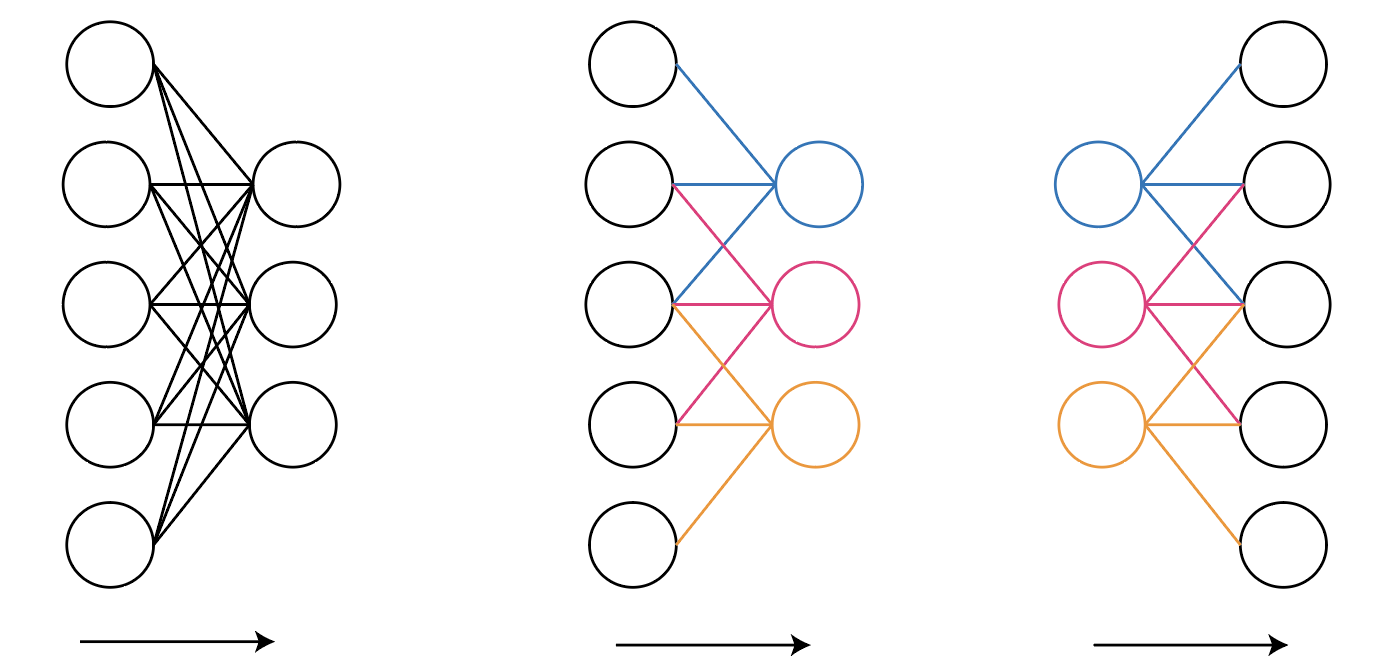
\includegraphics[width=5in]{images/cnnvsmlp.png}
    
    \caption{Multilayer Perceptron (left): each output from one layer is fed into the inputs of every node in the subsequent layer. Convolutional Neural Networks (middle) on the other hand have a 'receptive field', taking advantage of the spatial coherence of pixels in image data. The convolutional upsampling operation (right) is frequently used to upsample a low-dimensional feature space, to a higher dimensional one. It is often employed as a 'learned' information decompression.}
    
    \label{convexhull}
\end{figure}


Convolutional neural networks (CNN's) are similar to multilayer perceptrons, but introduce a spatial invariance that makes them particularly well suited for extracting high-level features from image data. Where multilayer perceptrons are densely connected, the connectivity pattern of each node in a CNN takes advantage of the hierarchical organisation of patterns in image data by using a 'receptive field'. Biologically inspired, these nodes respond to stimuli only in their receptive field, and so they typically learn to identify salient 'features' in the image - combinations of pixels that represent some kind of underlying structure. As these types of networks grow deeper, the features that they learn typically become more complex \cite{lecun1989cnn}. Early layers are provided with a small region of the image, typically a window between 3 and 11 pixels wide, and so will usually learn primitive features such as lines and corners. Deeper layers however may learn to recognise higher-level features such as eyes and mouths, and eventually even human and animal faces.



CNN's are thus popular 'feature extractors' in computer vision - their ability to learn to respond to different types of stimuli mean that they have been used as a dimensionality downsampling tool, taking the millions of dimensions present in digital images  and compressing them to a feature space with a much smaller number of parameters. Closely related is the convolutional upsampling operation which performs the inverse - taking a feature space and learning to upsample that feature space into something meaningful \cite{long2014fcn}. This has given rise to a particular topology of CNN called the encoder-decoder architecture, which will be useful throughout this thesis. The encoder part of a CNN is composed of a series of convolutional downsampling operations - this can be thought of as finding an efficient compression of the information stored in the image. The decoder subsequently uses this compressed form of the information to extract some meaningful information about it. One example where this architecture has been used is in \cite{long2014fcn}, which outputs a classification for each pixel in the image. In this thesis, a fully convolutional encoder-decoder architecture will be used for a similar purpose, but rather than classifying each pixel into one of several categories, it will regress depth values for each pixel. 

\chapter{Literature Survey}


\section{Depth Estimation and Visual Odometry}


\subsection{Geometric Approaches}

Since the invention of the pinhole camera, most cameras have captured 2D representations of a 3D world, meaning information about physical structure is lost. With the addition of a second viewpoint however we can learn a little more about the shape of the scene as governed by epipolar geometry \cite{zisserman2004multiview}. Meanwhile, a video is a sequence of images, taken in very quick succession, and so one could think of video footage as a multi-view camera where each image is separated not only spatially but also temporally. Identifying the amount of motion between two temporal frames of the video camera is the goal of visual odometry, where one intuitive approach is to observe the direction of movement of each pixel between the pair of images. In practice, features such as SURF \cite{bay2008surf} or SIFT \cite{lowe2004sift} features are used to simplify the search for image correspondences. The fundamental matrix, which describes the relationship between two cameras in space can then be estimated using techniques such as the 8 point algorithm. 

Doing so monocularly however is problematic because with a single camera there is no way of concretely discerning the actual magnitude of the movement based on pixel data alone, meaning some kind of scale factor needs to be estimated based on characteristics of the image \cite{gakne2018scale, nister2004vo, zhou2016scale, zhou2019scale}. In fact, this scale ambiguity is often exploited by film makers - what appears as a sweeping shot of a vast landscape on the big screen is often modeled as a miniature film set in the studio. Because the image is monocular, there is no way to ground our measurements of scale in real world units, and so we resort to our imaginations and learned experiences to fill in the gaps. What \textit{is} preserved in these monocular setups however is the overall structure of the scene and motion of the camera - we may not know how large the object is or how far the camera has moved, but we \textit{can} compute the  shape of the object as well as the direction of camera motion. 

Using a stereo pair of cameras with a known baseline however allows the scale ambiguity issue to be resolved. In the monocular approach, the fundamental matrix must be estimated to an unknown scale factor, however given two camera views of the same scene, features can be directly triangulated in 3D space. Corresponding these 3D points between the first and second pair of images allows the translation and rotation of the camera pair to be found by optimising a cost function to most closely match the two sets of 3D points. 

These approaches have demonstrated very strong results and indeed represent a strong foundation for computer vision in mobile robotics, however the question also arises, why should robotics be restricted to using cameras that mimic the human eye? Perhaps more information can be obtained if a different kind of camera is chosen? An alternative approach that utilises all of the pixel energy in the scene, takes advantage of the advanced geometric information available when the regular camera is swapped out for a plenoptic camera \cite{dansereau2011plenopticflow}. Utilsing this rich geometric information, \cite{dansereau2011plenopticflow} estimates a pixel-wise depth estimate using the gradient-depth constraint. Correspondences in 3D space can then be found, and pose can be directly solved for. The 'plenoptic flow' algorithm is an attractive approach for visual odometry as the computational complexity is constant with scene complexity, and the camera pose has a closed-form solution. \cite{dong2013plenopticflow} showed experimentally that the results obtained from using a plenoptic camera to perform visual odometry demonstrates superiority in terms of both computational complexity as well as accuracy.

Yet more complex imaging devices such as lenslet based plenoptic cameras and polydioptric cameras may yield even more useful information, boosting performance and reducing the amount of hard work, however interpreting the information from these cameras is not always obvious. This brings us to a data-driven appraoch that employs the pattern-recognising capabilities of machine learning algorithms to obviate the need for calibrating these complex imagers.


\subsection{The Machine Learning Approach}

One recent approach that has driven a large body of research is the use machine learning to perform both of these tasks, utilising convolutional neural networks to learn a non-linear mapping directly from a pair of images to their depth maps, as well as the relative pose between them \cite{eigen2014supervised, garg2016unsupervised,godard2016consistency, liu2015supervised, zhou2017unsupervised}. Combining the spatial awareness of the convolutional down sampling operation with a neural networks ability to learn accurate approximations for complex, non linear functions, these approaches have found success in both supervised \cite{liu2015supervised, eigen2014supervised}, and unsupervised settings \cite{garg2016unsupervised, godard2016consistency, zhou2017unsupervised}. In the supervised family of algorithms, \cite{eigen2014supervised} and \cite{liu2015supervised} take advantage of datasets such as KITTI \cite{dataset-kitti}, containing ground truth depth maps collected using state-of-the-art depth sensors and poses measured from inertial sensors. 

Unsupervised experiments such as \cite{garg2016unsupervised, godard2016consistency,zhou2017unsupervised} on the other hand exploit the constraints imposed by epipolar geometry to learn depth either by using known camera poses or by estimating pose in addition to depth. The general pipeline utilises two CNN's, one who's purpose is to predict dense per-pixel depth maps given a single image, and the other who's job is to estimate the 6 degree-of-freedom pose from the first frame to the second given both images.

\begin{figure}[htbp]
    \centering
    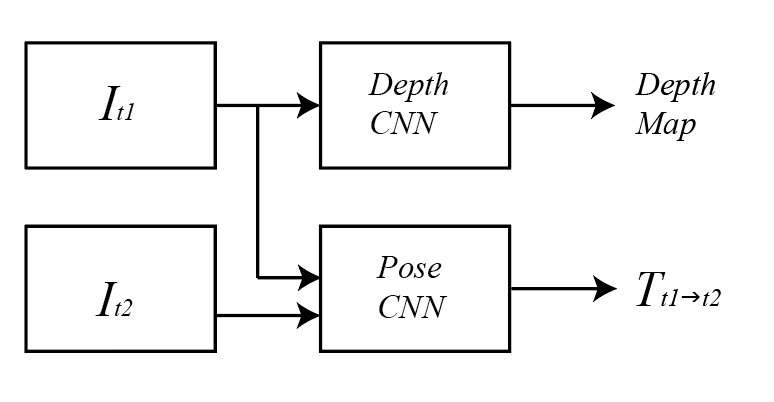
\includegraphics[width=3in]{images/cnns.png}
    \caption{Machine learning approaches have demonstrated strong results in simultaneously estimating depth maps and relative poses between images. Typically, a pair of CNN's is used, one for each task. The depth CNN is provided with the first view at $t=1$ and the pose CNN is provided both views.}
    \label{2cnns}
\end{figure}


While the training pipeline is unsupervised in the sense that labelled data is not required, some form of supervision signal is nevertheless required to optimise the parameters of the pair of networks. These papers take advantage of the fact that if the physical structure of a scene is known, then a novel rendering of that scene from a different viewpoint is achievable. Thus, \cite{garg2016unsupervised} suggested using photometric reconstruction as a supervision signal - from $I_{t2}$, reconstruct $I_{t1}$. The difference between the reconstruction and the real image can form a supervisory signal for the pair of networks. 


\begin{equation}
    L_{photometric} = \sum_n^W \sum_m^H |I_{t1}(m,n) - \hat{I_{t1}}(m,n)|
    \label{photometricloss}
\end{equation}


Humans can easily imagine what a scene will look like if we move our heads slightly, but only if we know the overall shape of the object we are looking at. Similarly, given two images separated by a small interval of time $I_{t1}$ and $I_{t2}$, one could synthesise what $I_{t1}$ would look like by sampling the pixels from $I_{t2}$, if the relative pose $T_{t1\rightarrow t2}$ between the two cameras and a pixel-wise depth of the scene $D_{t1}(p)$ is known. In practice, this can be done by obtaining the coordinates of the pixels in the first image $p_{t1}$ projected on to $I_{t2}$'s camera sensor. Assuming a pinhole model, the complete expression for $p_{t1}$'s projected location on the second camera, $\hat{p_{t2}}$ is 

\begin{equation}
\hat{p_{t2}} = KT_{t1\rightarrow t2} D(p_{t1}) K^{-1} p_{t1}
\end{equation}

where K represents the intrinsics matrix. In right-to-left order, this transform first maps each pixel to a ray direction using the camera intrinsics $K$. Each ray is then given a depth with the per-pixel depth map $D(p_{t1})$, producing a 3D point cloud. The transform $T_{t1 \rightarrow t2}$ transforms each point to the coordinate frame of the second camera, then the matrix $K$ projects each of those points onto the camera sensor of the second camera. The obtained coordinate $\hat{p_{t2}}$ is continuous, while pixel coordinates are discrete. A pixel value thus needs to be interpolated, keeping in mind that each step of a neural network pipeline must be differentiable to support the backpropagation of gradients. 

It was suggested in \cite{zhou2017unsupervised} that adopting bilinear sampling could be used as a fully differentiable sampling mechanism. The use of bilinear interpolation as a differentiable sampling pipeline was first proposed in \textit{Spatial Transformer Networks} \cite{jaderberg2015spatialtransformer}, and adapted by \cite{zhou2017unsupervised} to perform the differentiable image warp. A bilinear sampling kernel is described by 

\begin{equation}
    V = \sum_n^W \sum_m^H U_{nm} max (0, 1-|x - n|) max(0, 1-|y - m|)
\end{equation}

Where $V$ is the output of the sampling kernel, $U$ is the source image being sampled, $n$ and $m$ index over the columns and rows of the kernel respectively, $H$ and $W$ are the height and width of the sampling kernel, and $x$ and $y$ are the local coordinates of the sampling location. The $2 \times 2$ sampling kernel used to perform the photometric reconstruction is, in essence a weighted sum of the 4 nearest neighbour pixels, based on its proximity to those pixels. The equation is differentiable with respect to both x and y:


\begin{equation}
    \frac{\partial{V}}{\partial{x}} = \sum_n^W \sum_m^H U_{nm} max(0, 1-|y - m|)
\end{equation}
\begin{equation}
    \frac{\partial{V}}{\partial{y}} = \sum_n^W \sum_m^H U_{nm} max(0, 1-|x - n|)
\end{equation}

Using this bilinear sampling kernel, we can thus sample pixels from $I_{t2}$ to reconstruct $I_{t1}$ in a fully differentiable manner, allowing the backpropagation of gradients through the networks. The pipeline with photometric reconstruction as the supervision signal can be illustrated as shown in figure \ref{supervisedMLCNNS}.


\begin{figure}
    \centering 
    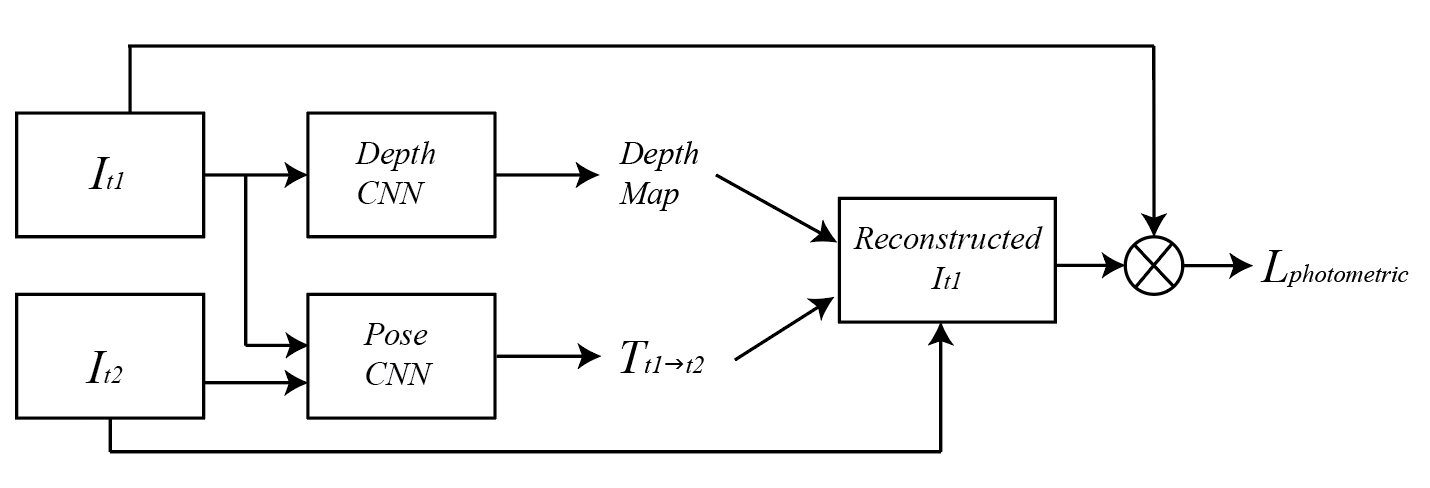
\includegraphics[width=5in]{images/mlpipeline.png}
    \caption{To provide a supervisory signal to the depth and pose CNN's, \cite{garg2016unsupervised} suggested using photometric reconstruction. The loss function is formulated by taking the difference between the reconstructed image $\hat{I_{t1}}$ and the actual image $I_{t1}$, shown in equation \ref{photometricloss}.}
    \label{supervisedMLCNNS}
\end{figure}


In addition to the photometric reconstruction loss providing the main supervision signal to the network, \cite{zhou2017unsupervised} employs a smoothness loss to ensure that the produced depth map is globally smooth. The smoothness penalises the second order gradient of the image - i.e. the depth network is encouraged to produce a depth map characterised mostly by low-frequency components, and penalised for high-frequency components. Recognising that depth discontinuities frequently occur in parts of the image where a strong edge appears, \cite{godard2016consistency} on the other hand suggested the use of an edge-aware smoothness loss that also penalises large gradients in the depth map $\partial{d}$, but lowers the weight of the loss in regions where the image gradient $\partial{I}$ is large. 

\begin{equation}
    L_{smooth} =  \sum_n^W \sum_m^H |\partial_x d_{nm} e^{-|\delta_x I_{nm}|}| + \partial_y d_{nm} e^{-|\delta_y I_{nm}|}|
\end{equation}

There have been several iterations \cite{godard2016consistency, godard2018selfsupervised, zhan2018deepfeature} of this pipeline, most of which have focussed on introducing novel loss functions to improve the quality of the depth and pose estimates. To the best of our knowledge however, this pipeline has only ever been applied to monocular and stereo camera setups. While monocular and stereo cameras are ubiquitous in modern digital devices, this thesis will investigate the potential for the use of this pipeline to achieve improved results using a broader, more generalised family of imaging devices. 

Breaking free of the pinhole principle from which human eyes have developed and which commercial cameras have adopted, has wide implications in the field of machine vision. Reinforcing this idea is the rise in popularity of imaging techniques such as multi-spectral imaging, plenoptic cameras and polydioptric cameras, however interpreting ray directions and geometry for new cameras may not always be apparent, giving rise to the data-driven approach. Working on the principle that machine vision does not necessitate mimicking the human eye to capture imagery, this thesis investigates the capabilities of machine learning for querying depth and visual odometry using one such novel imaging device - a camera array.



\section{Convolutional Neural Networks and Light Field Images}

In order to craft such a machine learning pipeline that complements the use of camera arrays, an investigation into input methods for 4D light fields into convolutional neural networks is due. It is recognised in \cite{sun2016lfdepthcnn} that while epipolar plane images (EPI) explicitly encode depth information, directly extracting such information without significant post-processing refinement and computational cost is difficult. \cite{sun2016lfdepthcnn} demonstrates strong results in using a CNN to interpret the gradient-depth relationship between an EPI and the images corresponding depth map. An EPI is extracted in both the horizontal and vertical direction for every row and column of the image in the $u, v$ plane, and subsequently fed to the network as two long, cubic volumes to obtain their results.

The rich textural data available in a 4D lightfield was purposed by \cite{wang2016lfcnn} for the task of material recognition using a deep CNN. In addition to reporting significantly improved material-recognition results (from 70\% to 77\% accuracy), \cite{wang2016lfcnn} proposes and compares a number of strategies for training on 4D images. One method that achieves strong results uses an angular filter, taking advantage of the 'angular resolution' that is gained by using a light field image over 2D images. The 4D light field image is first reshaped to form what \cite{wang2016lfcnn} calls a 'remap' image. To illustrate what a remap image looks like, a traditional 2D image is formed by discrete pixels, whereas a remapped 4D image on the other hand is formed of blocks of pixels, each block of size $h_a \times w_a$, formed by taking one pixel from each camera in the array. The result is a 2D image from which a 2D convolutional filter is able to learn features that indicate texture and parallax. While the remapping method achieved the best results, unfortunately such an arrangement of the image data does not make sense in the case of the camera array being used for this project as the cameras are arranged in a crosshair formation - 8 vertical cameras, 8 horizontal and 1 center image. The remapped image using this camera would comprise $17 \times 17$ blocks of mostly black pixels, producing a very inefficient representation of the data. 

Another method proposed in \cite{wang2016lfcnn}, albeit one that demonstrated lower accuracy than the angular filter method, was to concatenate images along their RGB channels prior to being fed to the network. The dimensionality of the image is quickly downsampled, and is thus a more computationally and memory efficient method than using angular filters, whilst still demonstrating improvement over 2D images. A potential improvement on this strategy that may prove useful in this work would be to use a dilated convolution, effectively opening the receptive field to a much larger area of the image without increasing computational complexity. Such a CNN would benefit from being able to sample a larger area of the image to recognise robust geometric features. 

These strategies each treat light field images as a volume of 2D images, and thus do not take full advantage of the 4D signal structures present in a light field. One possible improvement that might learn to more effectively utilise these 4D signals is to swap out the 2D convolutional filters typically used in image data for a 3D convolutional filter which is more commonly applied to video data. 


\chapter{Progress Report}

In this first semester of this thesis project, I've focussed my energy on two core objectives: data collection, and building a pipeline on paper. Furthermore, preliminary results using the KITTI benchmarking dataset have demonstrated promise that the objectives of this thesis are achievable, and will indeed produce knowledge worthy of contribution to the discussion on computer vision in robotics. This section describes the methodologies of the tasks undertaken so far, the preliminary results that have been attained, and an updated research proposal outlining the objectives, planned experiments and an evaluation framework for the remainder of this project.

\section{Data Collection}

\subsection{Ground Truth Pose Data}

\begin{figure}[h]
    \centering 
    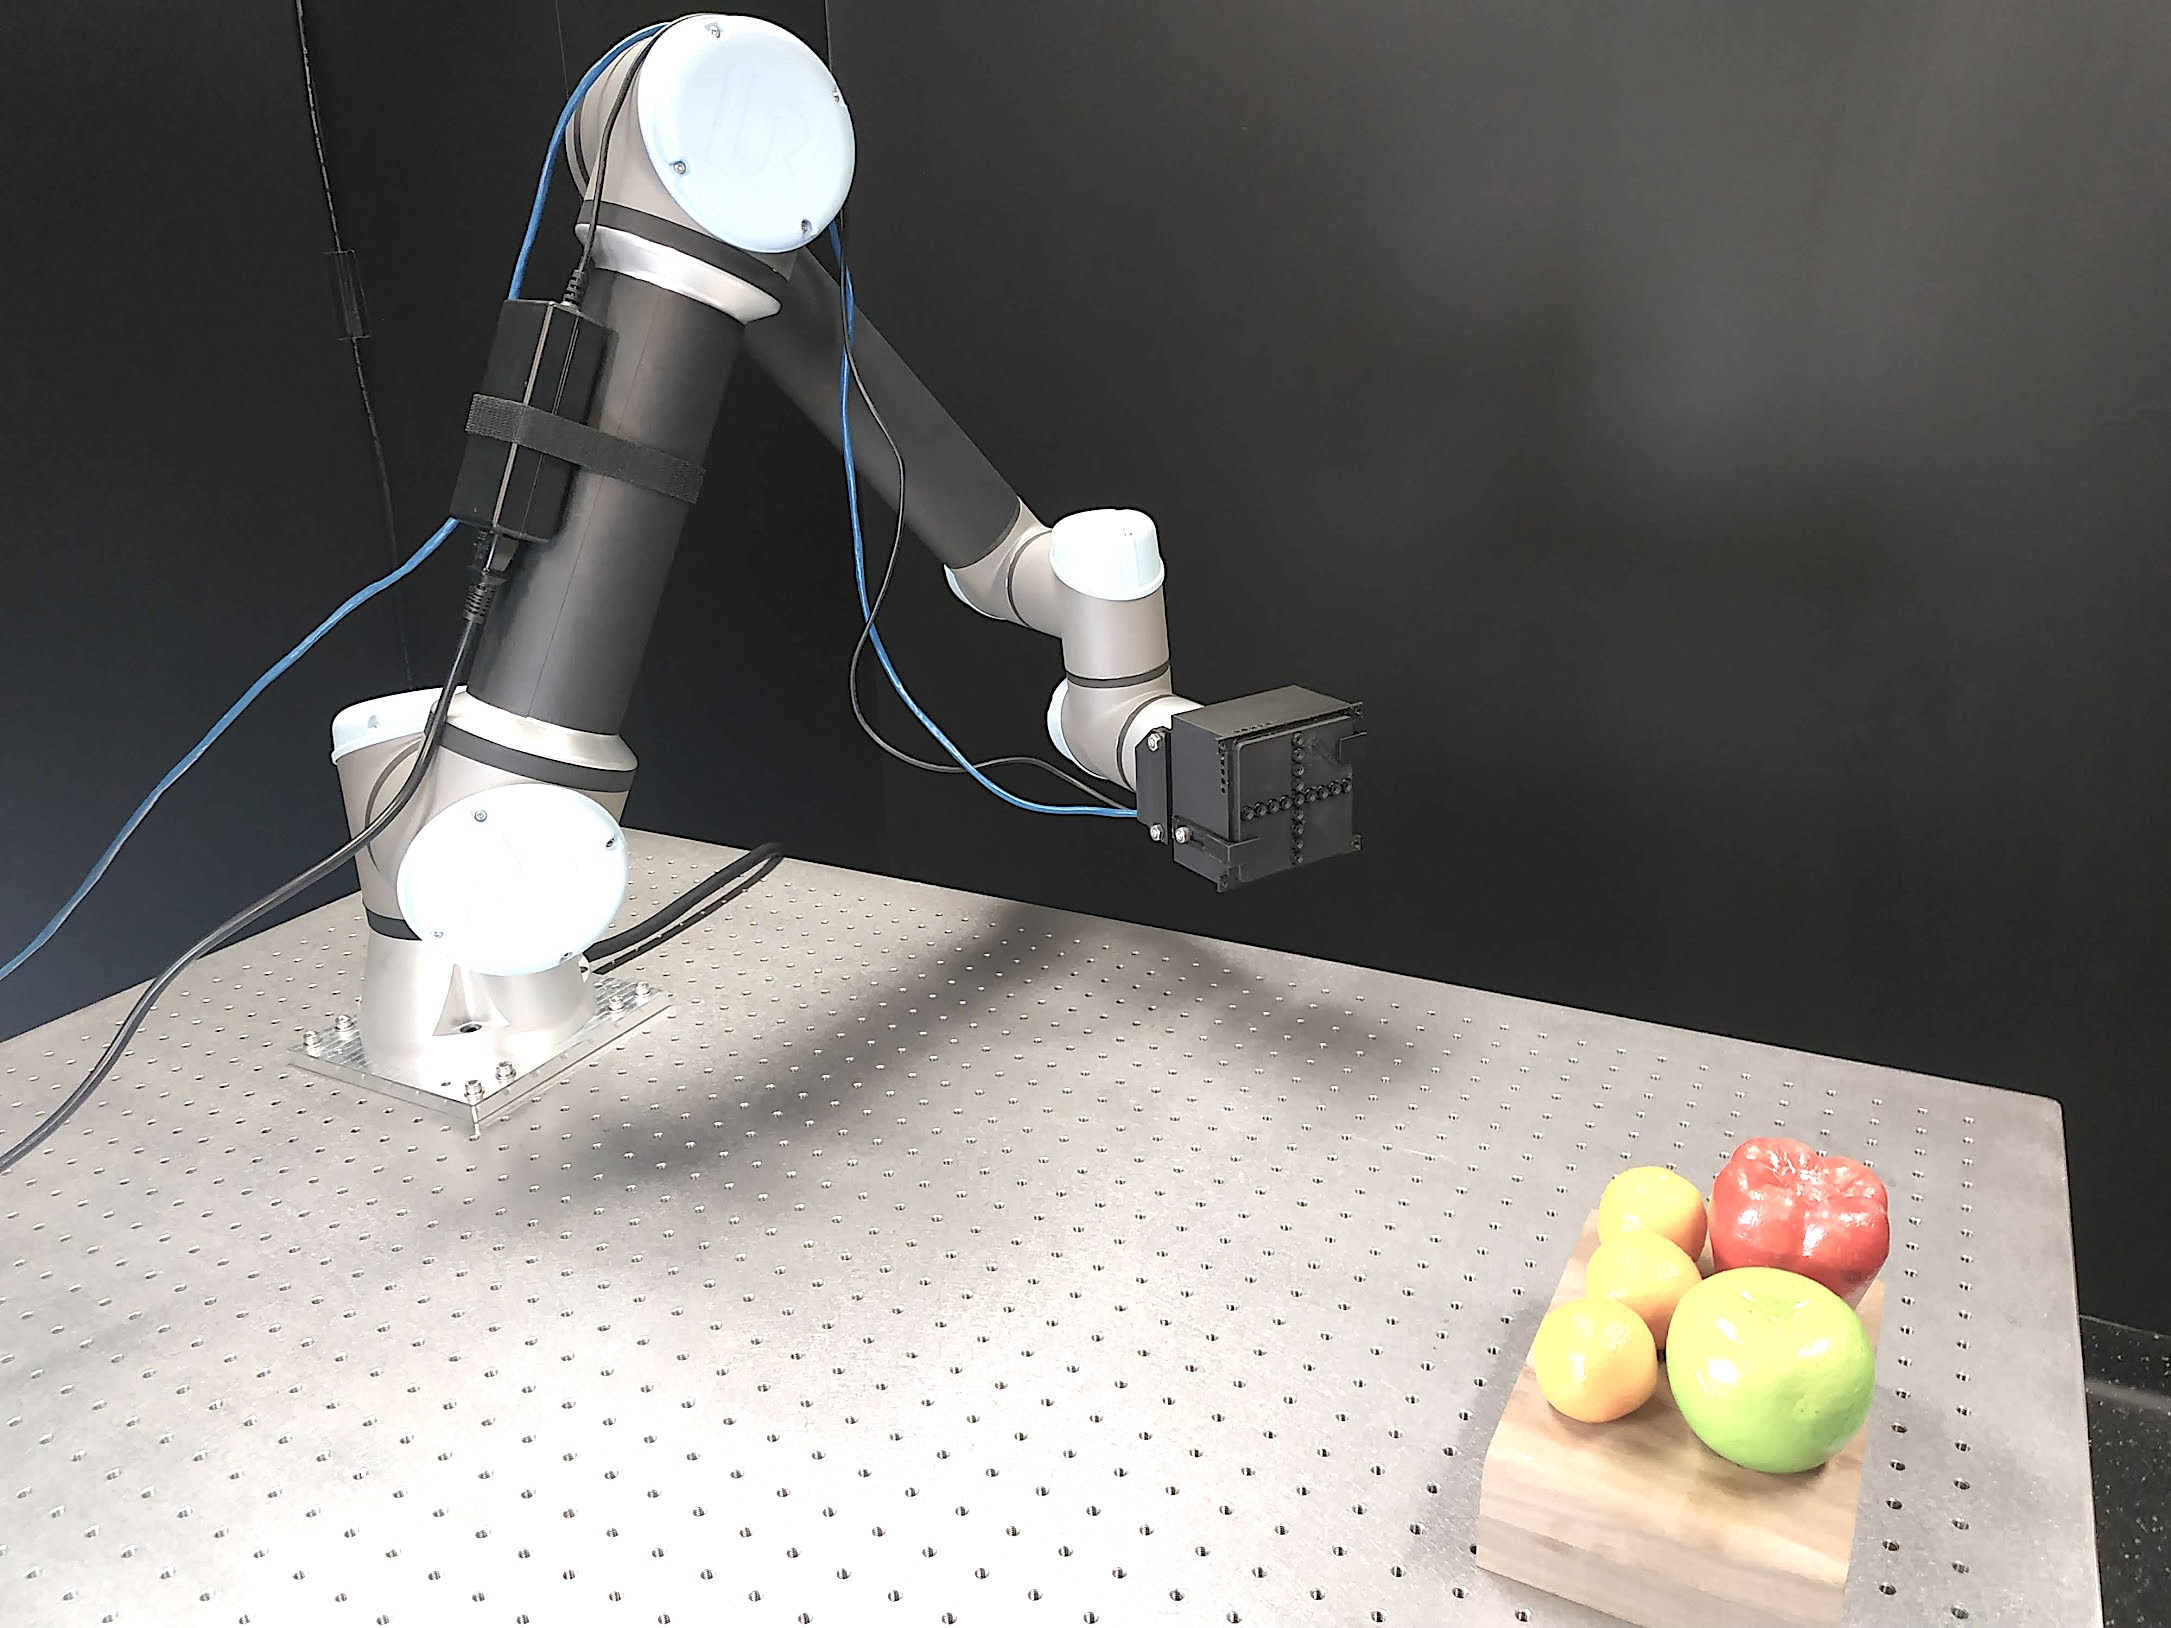
\includegraphics[width=4.5in]{images/experimentalsetup2.jpg}
    \caption{The experimental setup utilises a Universal Robots UR5E robotic arm to precisely measure ground-truth pose to allow effective evaluation of the projects visual odometry results.}
\end{figure}

Important to the success of this project will be a strong evaluation framework. Existing datasets such as KITTI and CityScapes benefit from state-of-the-art sensor equipment including inertial sensors and lidar, allowing researchers to effectively benchmark their results. Similarly, this project places a strong emphasis on validation using ground truth data. One of the primary tasks that will be evaluated is visual odometry, and so ground-truth pose for each image will be a valuable resource. In this project, pose is collected by attaching the camera to a Universal Robots UR5E robotic arm, which is capable of sensing to a high degree of accuracy the pose of the end effector. Furthermore, the UR5E is able to perform accurate movements and trajectories with payloads of up to 5 kilograms, making it a suitable robotic mount for the camera. 

A challenge that needed to be solved prior to data collection was thus coming up with the means of attaching the camera to the end effector. The UR5E uses a standard interface plate for attaching end-effectors such as grippers and other tools. The camera on the other hand, as an early prototype, does not have any mounts available on the market for attaching it to the robot. A suitable mount therefore needed to be fabricated, taking into consideration the cameras ventilation and electronic connection requirements. A two-piece mount was designed using SolidWorks, and fabricated as a 3D printed component with polylactic acid (PLA) filament, allowing easy mounting and dismounting to the robot using standard M6 bolts. 

Another important aspect of this data-collection methodology is querying and storing pose data from the robot. A client library was written in python, which establishes a TCP/IP connection with the robot over the local network, allowing both movement commands to be sent to the robot, and feedback data about the end-effector's pose to be streamed back to the client PC. The client library also provides functionality for pre-computing trajectories and joint angles, using the PyBullet physics engine and the known kinematic model of the robot. One useful trajectory function from the client library procedurally generates new waypoints with a stringent collision-checking mechanism, meaning data-collection can be performed autonomously. A challenge that has prevented a fully autonomous footage collection routine has been working with non-timestamped image data. The particular imaging setup currently provides only enough bandwidth for image data at 0.5 frames per second. Furthermore, the onboard rectification processes take several seconds to complete, and what's more, because the on board storage of the camera is limited, the image must be streamed over an ethernet connection to a PC taking several more seconds. The actual time that the image is captured is therefore ambiguous and so correlating each image with a pose-stamp is difficult. An intermediate solution has been to manually control the arm to each waypoint, and pausing while an image is taken and the pose is saved. 

\subsection{Imagery}

The specific imaging device being used is manufactured by EPIImaging, and consists of 17 subapertures. The communication interface with the camera is a network connection serving image data over the HTTP protocol via a straightforward URL request. Both rectified and unrectified images can be requested, and the format of the returned image data is a $17\times 3 \times 1024 \times 968$ block of bytes representing pixel data from each of the 17 image sensors. A simple client library was written in python that automates the URL request, and subsequent decoding of image bytes, allowing data to be collected quickly and conveniently.

\section{Proposed Pipeline}

This thesis project will utilise a similar depth estimation and visual odometry pipeline to that described in section 3.1, with the main point of difference being the dimensionality of the input images. Given two sequential light fields of a scene, the pipeline will estimate the relative pose, as well as dense depth maps for each, and use photometric reconstruction error as the supervisory signal. Rather than use two independent CNN's however, a single CNN backbone will be used to predict both depth and pose, localising knowledge of both tasks within one learned module. As explained in section 3.1.1, the tasks of depth and pose estimation are intricately related by geometry, and separating the two tasks into independently learned modules means that geometric information learned by one module is isolated from the other - sacrificing information transfer that could benefit both. As such, this thesis proposes using a single backbone encoder CNN with two decoder 'heads'. The first head will use the convolutional upsampling operation to regress pixel-wise depth values (producing $N$ depth maps of shape $H\times W$ where $N$ is the number of views in the camera array), while the second will transform the feature space learned by the encoder into a 6 degree-of-freedom pose estimate. The input to the backbone will be the two light field images $LF_1$ and $LF_2$. 


The image warp procedure will be as follows. Each pixel of each subaperture of $LF_1$ will be projected to a 3D point cloud using the known camera intrinsics and estimated depth values. Picking a single pixel $p1 = [s,t,u_1,v_1,1]^T$ from the first light field, and its corresponding depth estimate $D(p1)$, its projected point in 3D space is

\begin{equation}
    Q_{p1} = D(p1) K^{-1}[u_1,v_1,1]^T
\end{equation}

The 3D coordinate $Q_{p1}$ can then be projected to the pixel coordinate $p_2 = [s,t,u_2,v_2]$ of the second light field if the rigid transform $[R|t]$ from the first light field to the second is known.

\begin{equation}
    p_2 = K[R|t]Q_p
 \end{equation}

 We have taken a single pixel from $LF_1$ and projected it to the corresponding pixel and subaperture if $LF2$. In order to photometrically reconstruct $\hat{LF_1}$, we can simply populate the pixel $LF_1(p1)$ with the value at $LF_2(p_2)$. In the case where $p_2$ is not an integer number, which will be almost every time, bilinear interpolation can be used as a differentiable sampling mechanism, as described in section 3.1.2.

 \begin{figure}
    \centering 
    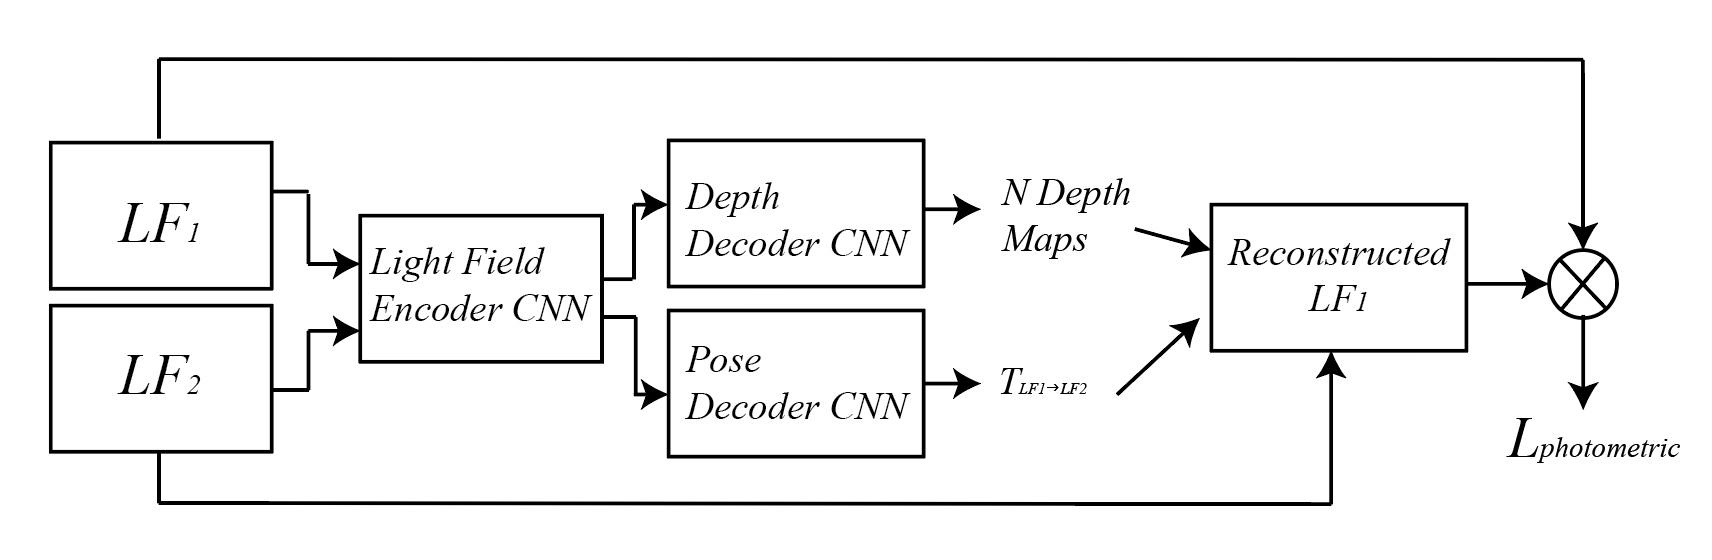
\includegraphics[width=5in]{images/lfpipeline.png}

    \caption{The proposed pipeline that adapts \cite{zhou2017unsupervised}'s monocular visual odometry and depth pipeline for light field images. The main differences are the dimensionality of the input - rather than monocular images, light field images will be used. Additionally, rather than learning two independent CNN's, a single encoder CNN will centralise knowledge of geometry in one learned module that can be queried with a depth decoder and a pose decoder.}
 \end{figure}

The supervision signal for the network will be the sum of the photometric reconstruction loss (equation 3.1), and the regularising edge-aware smoothness loss (equation 3.2). 

\begin{equation}
L = L_{photometric} + L_{smooth}
\end{equation}


\section{Updated Research Proposal}

With the benefit of 4 months of essentially non-stop thinking about the objectives of this thesis project, it is worth updating the original research proposal to reflect the evolution of the project. In those 4 months, the objectives of the thesis have not changed: namely performing depth and visual odometry using a camera array device. What I've continued to develop and refine in those 4 months however, is the motivation.

\subsection{Motivation}

Motion and depth estimation are important outcomes for the advancement of mobile robotics. The ability to perceive the structure of the space inhabited by the robot is imperative to its ability to navigate and interact with that space. Furthermore, a robots ability to maintain awareness of the physical pathways they have taken through space is advantageous in robots that are required to perform simultaneous localisation and mapping (SLAM). There are an extensive number of techniques and sensors currently being used to capture the 3D geometry of the world. One approach is to use time-of-flight cameras which emit modulated light signals, subsequently decoding the reflected light to compute pixel-wise depth estimates. Similarly, lidar uses intermittent laser pulses to reconstruct the surrounding 3D geometry. These sensors usually provide robust depth measurements, but some conditions such as glare and reflective/refractive surfaces can make their use prohibitive. Meanwhile, cameras are becoming cheaper while our signal processing bandwidth continues to improve, making visual based algorithms an attractive alternative.

A recurring question throughout this project has been, why use machine learning? Deep learning in computer vision and pattern recognition has drawn a lot of attention due to its impressive capabilities. Throwing machine learning at a computer vision problem in the hopes that it will work however, I feel is a dangerous mindset to adopt. Reflecting on this, I've found two convincing motivations for the use of machine learning as a mechanism for the depth estimation and visual odometry in this thesis project. The first idea is one that I've tried to interleave throughout this progress report, and revolves around the fact that machine vision is starting to see an uptick in non-traditional imaging techniques and novel optical designs. While these new ways of acquiring visual data means that new, unconstrained ways of thinking about cameras are emerging, the complex signal processing algorithms required to make sense of that data are not always obvious. Data-driven approaches have made a huge impact in computer vision, because they are capable of approximating complex functions and are capable of extracting patterns from high dimensional data. A data-driven approach, provided with the right kind of supervision signal may be one solution to the signal processing problem when working with novel imaging devices. So while the EPIImaging camera array is a simple extension upon the stereo camera pair, and a number of well established algorithms exist for working with multi-view imaging devices, it represents a new family of imaging devices that hasn't yet been fully explored from the signal processing point of view. 

The second idea is in situ, self-supervised learning. The ability for robotics to learn on the fly without any direct supervision from a human is attractive. As engineers, we like to make sure that the things we build are robust to different environments, but we usually end up having to fix them anyway when they break. But what if that environment is Mars and there aren't any engineers around? A machine that learns to work with what is available to it is thus an important step towards fully autonomous mobile robotics. The EPIImaging module is equipped with 17 subapertures, meaning 17 individual cameras must fail before all visual data is lost. Instead of hand-crafting algorithms that work on all possible permutations of 17 cameras arranged on a cross hair, wouldn't it be useful if the machine could learn to utilise the available data to it, without the requirement of an engineer being there?

\subsection{Updated Project Timeline}
The main tasks to complete before performing any experiments is to collect a critical mass of data. Comparable studies such as \cite{zhou2017unsupervised} use a dataset of around 30,000 images, however early experiments can begin with as few as 1000 datapoints. I expect to complete data collection in the next 4 weeks, and I'll be simultaneously developing the proposed algorithms from section 4.2 in software. One proof-of-concept experiment that will be performed in the coming weeks will be a fully-supervised visual odometry pipeline that trains a CNN to output relative pose data. This will be a strong first step in demonstrating the advantage of light field imaging for the objectives of this thesis, and will further serve as a rigorous, early test of the software building blocks from which the remainder of this thesis will build upon. 


\newpage

%\newpage
\bibliographystyle{plain}
\bibliography{bibliography.bib}

\end{document}
